%% ---------------------------------------------------------------------
\section{Design methodology and technical justification}
\label{sec:design}

\subsection{Trade study of GPS-denied navigation modalities}
\label{sec:design-trade}

Fifteen candidate approaches were screened (\cref{tab:solutions}) on drift (percent
of distance travelled), power, mass, update rate, range and cost in Indian rupees.
The values are concept-phase, literature-typical estimates
(\code{docs/ANALYSIS_SOLUTIONS.md}), not measurements. \Cref{fig:trade} summarises
them; further views are in \cref{app:trade}.

\begin{table}[H]
\centering\scriptsize
\caption{Screening data for the 15 modalities (mid-range values; ranges in
\code{docs/ANALYSIS_SOLUTIONS.md}).}
\label{tab:solutions}
\renewcommand{\arraystretch}{1.1}
\begin{tabularx}{\textwidth}{r L r r r r r}
\toprule
\# & \textbf{Modality} & \textbf{Drift (\%)} & \textbf{Power (W)} & \textbf{Mass (g)} & \textbf{Rate (Hz)} & \textbf{Cost (kINR)} \\
\midrule
1 & 2D LiDAR + optical flow & 1.4 & 7.0 & 150 & 75 & 12.5 \\
2 & Stereo camera V-SLAM (Pi~5) & 0.3 & 10.5 & 85 & 40 & 18.0 \\
3 & 2D LiDAR + monocular RGB & 1.5 & 8.0 & 140 & 35 & 15.5 \\
4 & Event camera odometry & 1.4 & 5.5 & 42.5 & 750 & 45.0 \\
5 & Visual SLAM & 0.3 & 17.5 & 85 & 40 & 12.0 \\
6 & Ultrasonic array & 2.5 & 1.25 & 27.5 & 30 & 16.5 \\
7 & Optical flow + rangefinder & 3.5 & 2.0 & 25 & 75 & 7.75 \\
8 & ArUco / fiducial tags & abs.\ $\pm$2\,cm & 2.0 & 20 & 20 & 5.0 \\
9 & Three RGB cameras (Pi~5) & 0.65 & 13.0 & 105 & 22.5 & 14.0 \\
10 & Depth camera (Pi~5) & 1.0 & 10.0 & 70 & 22.5 & 26.0 \\
11 & 3D LiDAR SLAM (Pi~5) & 0.125 & 22.5 & 375 & 15 & 425 \\
12 & FMCW mmWave radar & 2.0 & 7.0 & 120 & 35 & 77.5 \\
13 & UWB beacons & abs.\ $\pm$2\,cm & 2.0 & 20 & 75 & 30.0 \\
14 & Magnetic anomaly (MAGNAV) & 0.6 & 3.5 & 70 & 20 & 40.0 \\
15 & Terrain matching (TERCOM) & 0.45 & 10.0 & 225 & 12.5 & 235 \\
\bottomrule
\end{tabularx}
\end{table}

\begin{figure}[t]
\centering
\begin{subfigure}[t]{0.49\textwidth}
  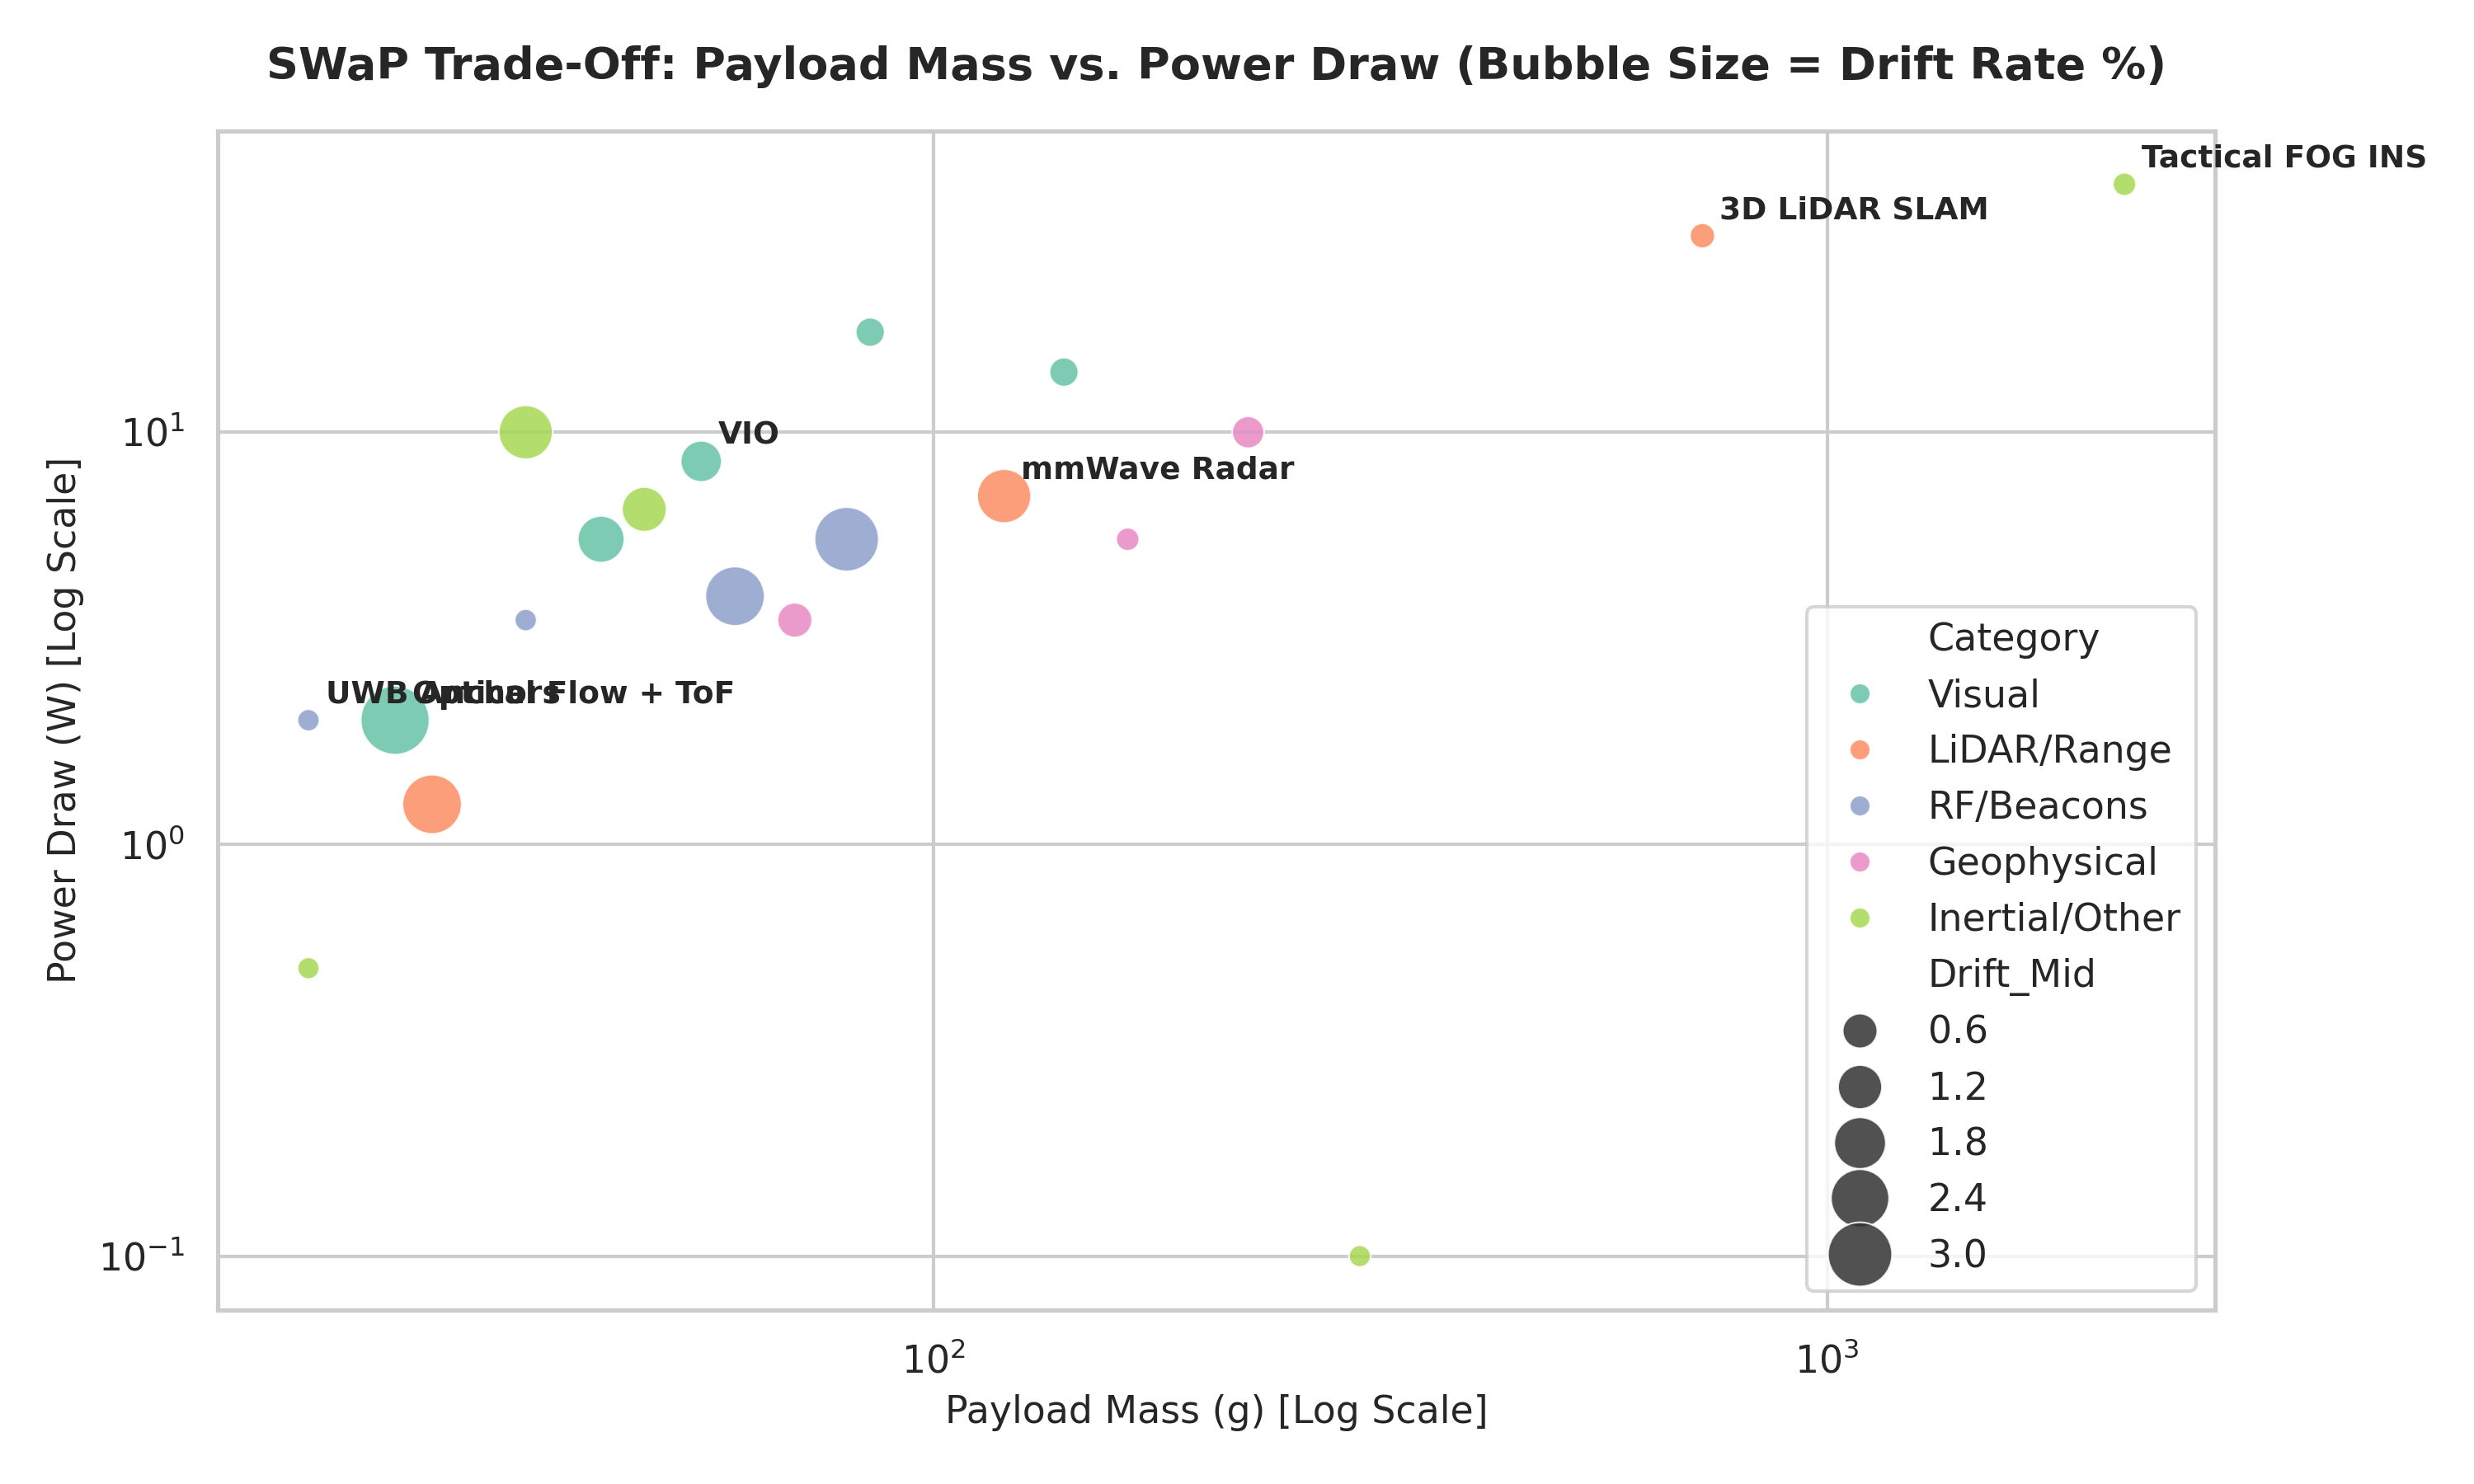
\includegraphics[width=\linewidth]{1_swap_tradeoff.png}
  \caption{SWaP trade-off (bubble size = drift).}
\end{subfigure}\hfill
\begin{subfigure}[t]{0.49\textwidth}
  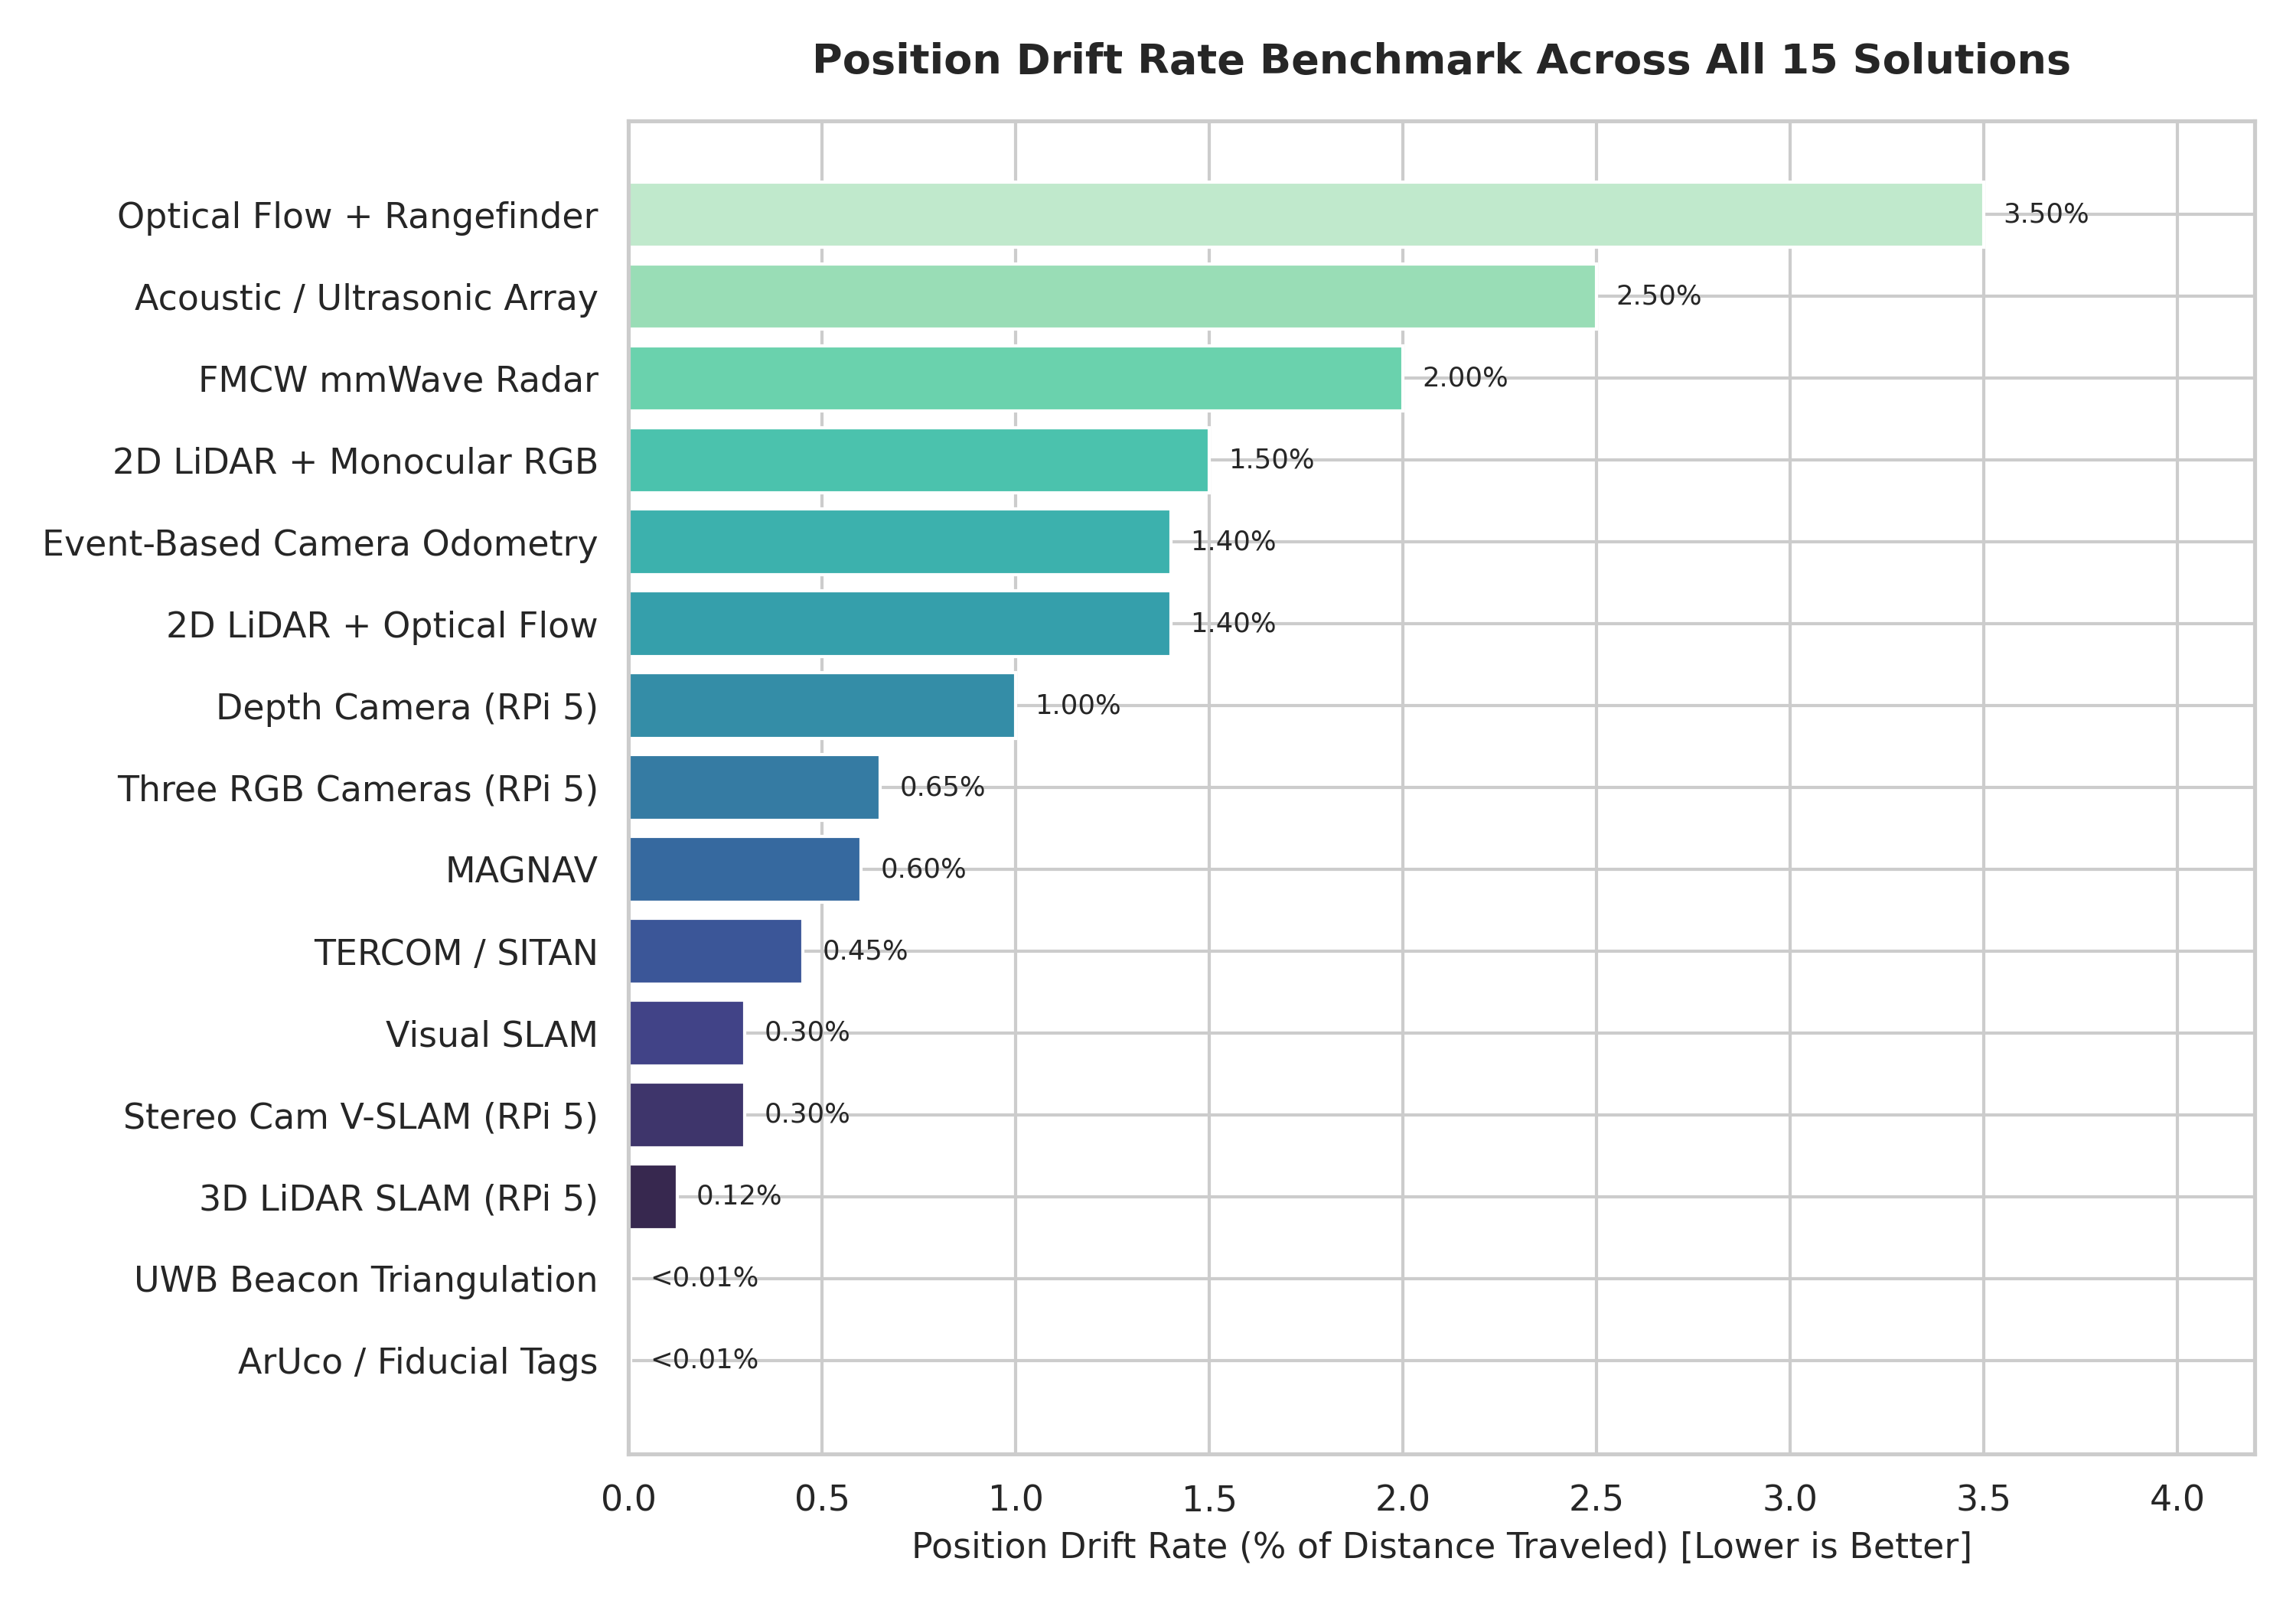
\includegraphics[width=\linewidth]{2_drift_rate_comparison.png}
  \caption{Drift rate ranking.}
\end{subfigure}

\vspace{2mm}
\begin{subfigure}[t]{0.49\textwidth}
  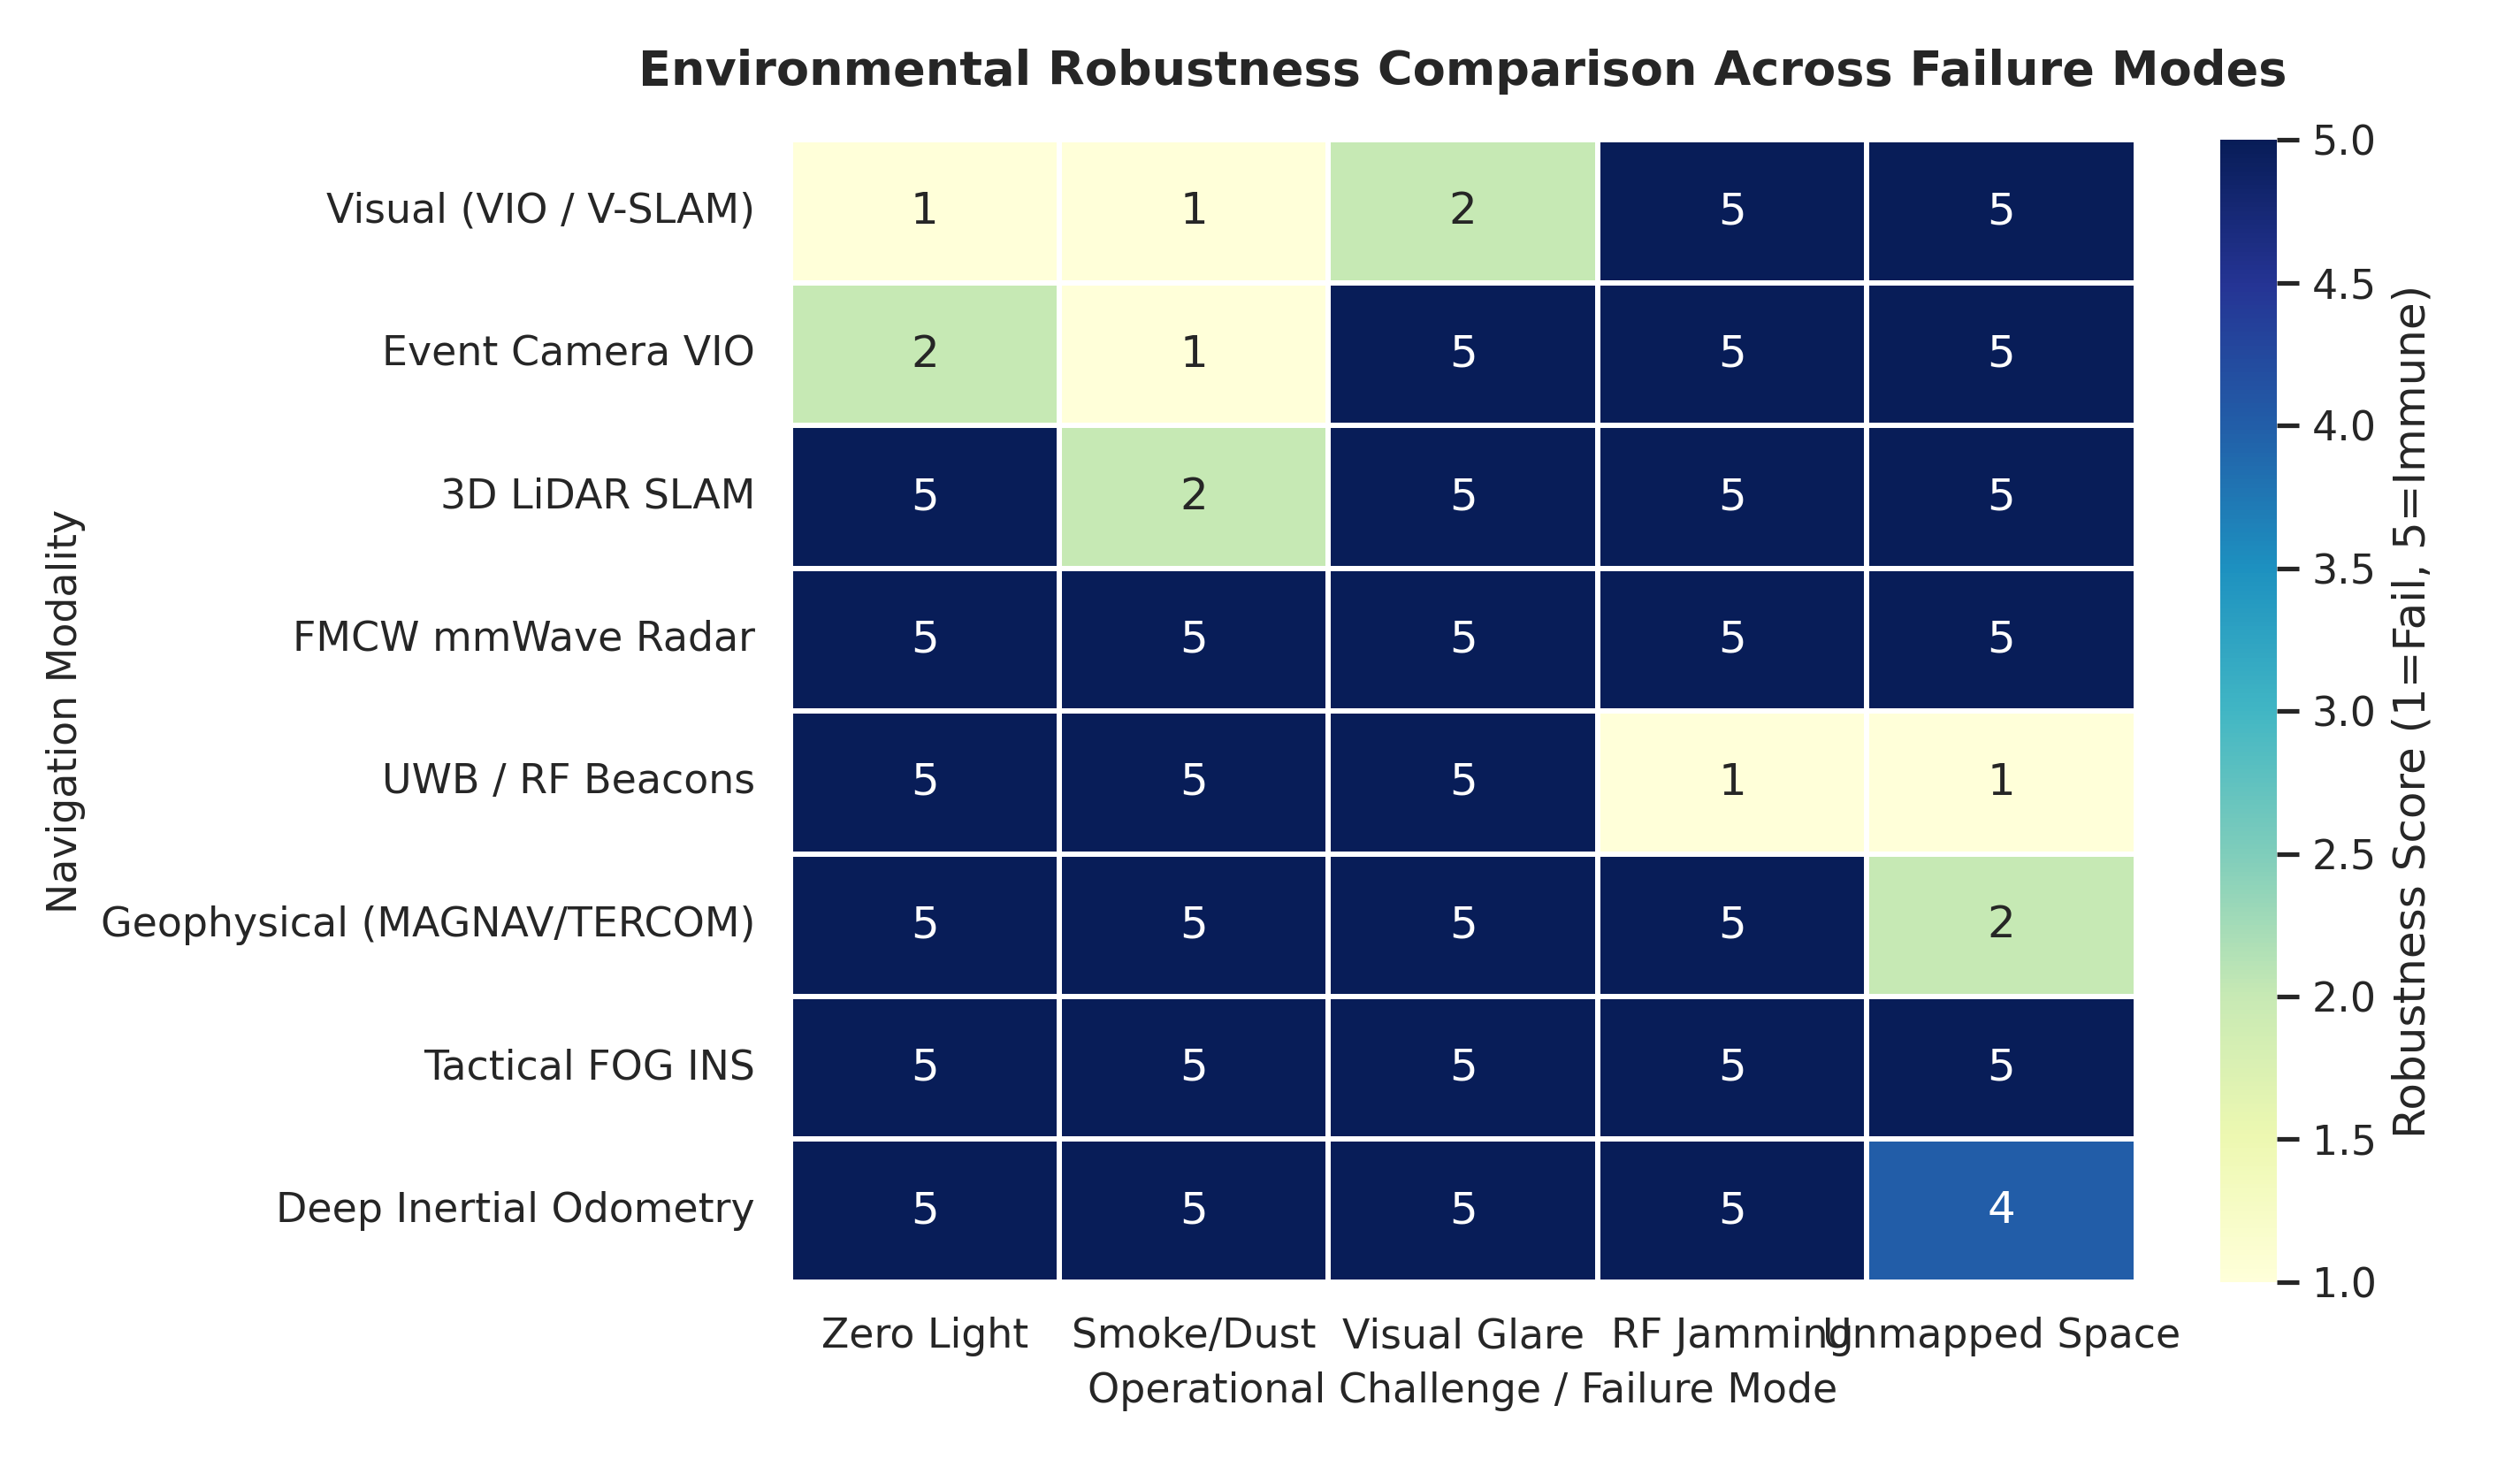
\includegraphics[width=\linewidth]{4_robustness_heatmap.png}
  \caption{Environmental robustness (1 = fails, 5 = unaffected).}
\end{subfigure}\hfill
\begin{subfigure}[t]{0.49\textwidth}
  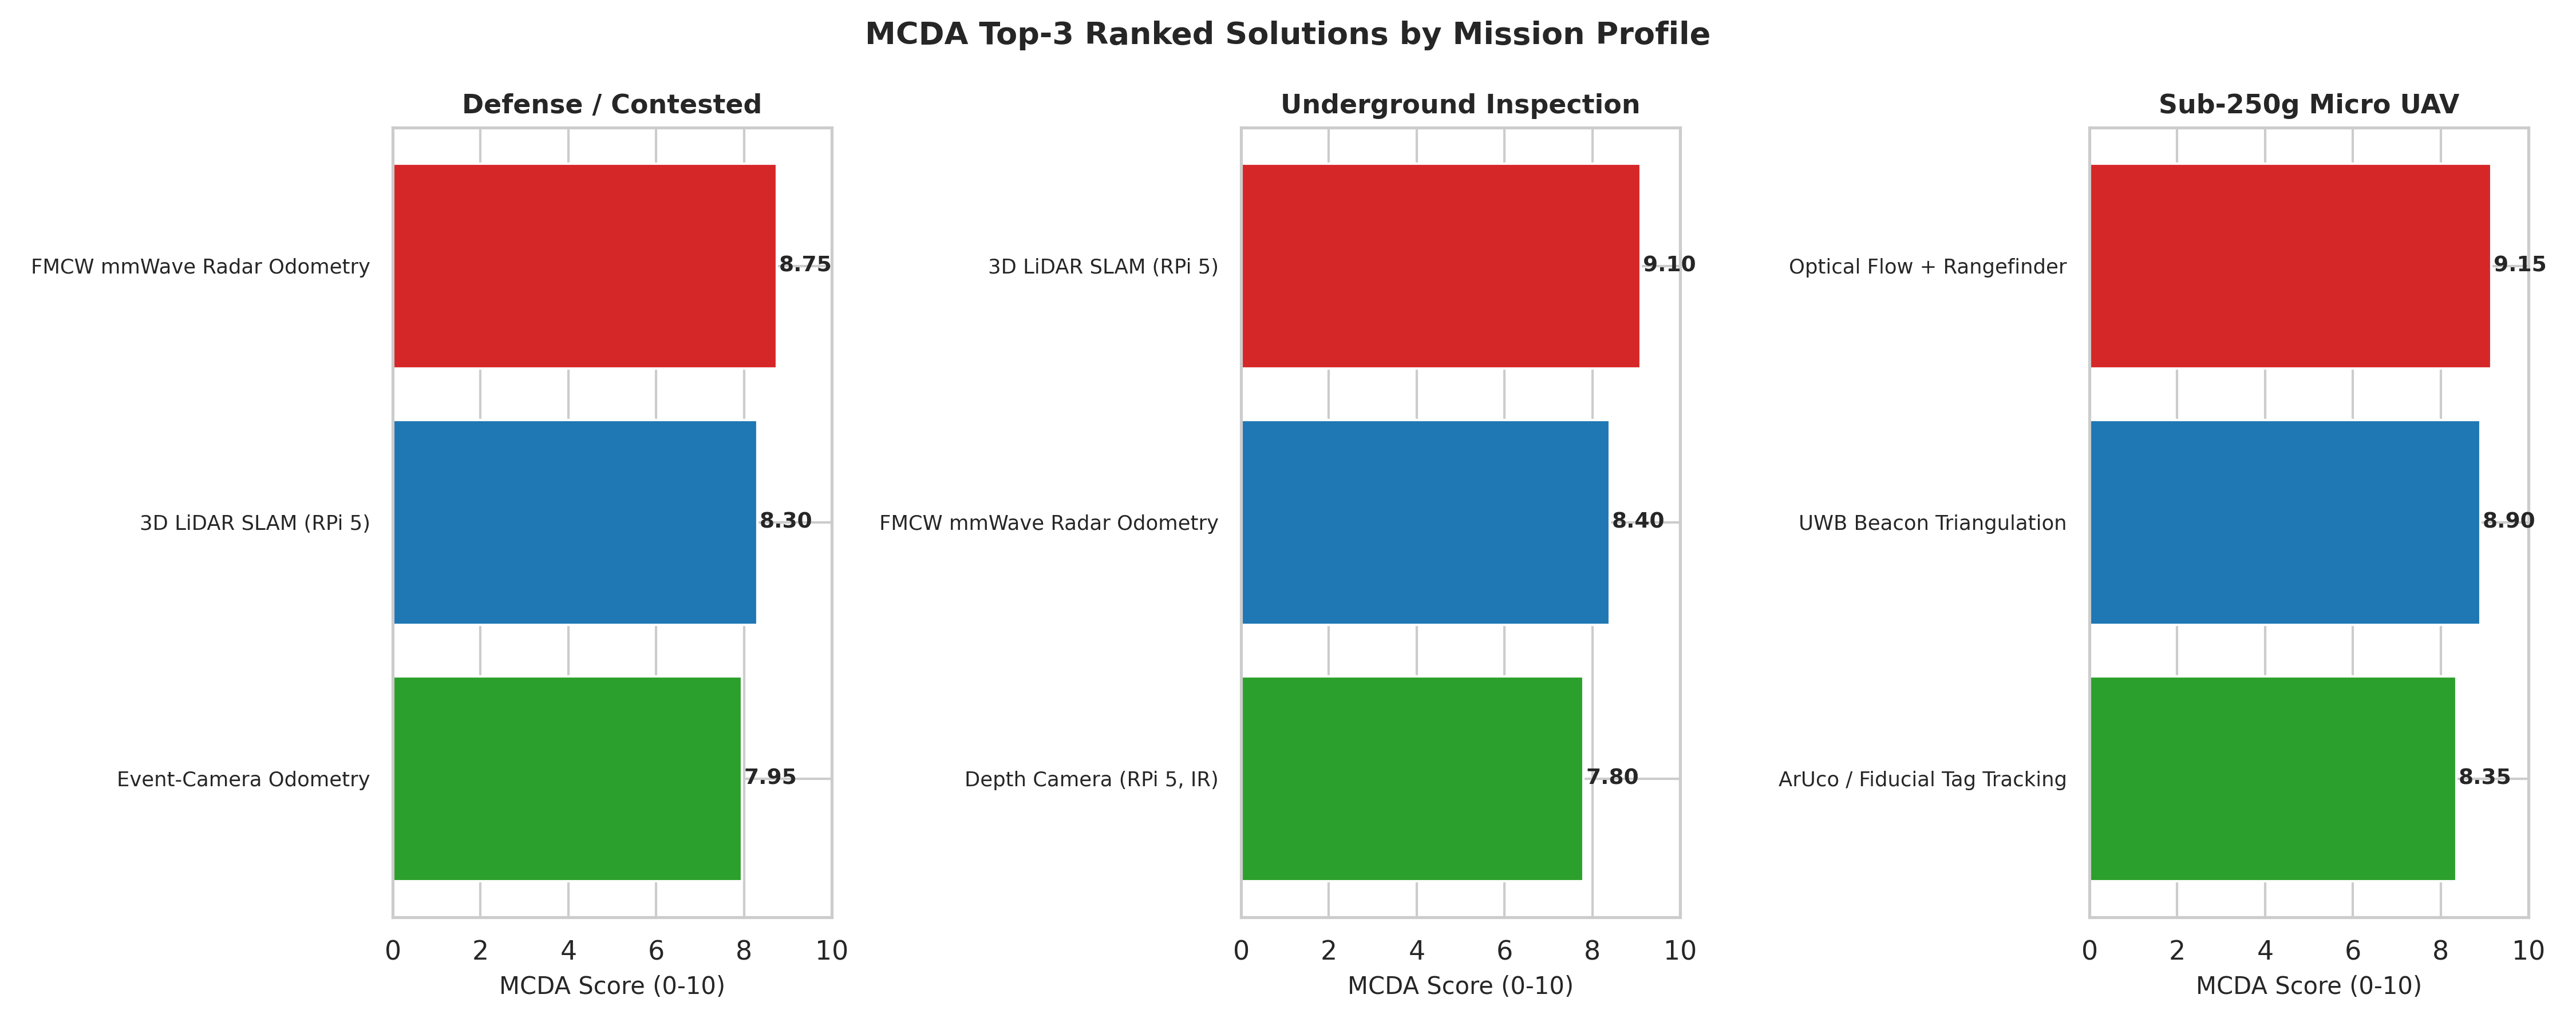
\includegraphics[width=\linewidth]{12_mcda_scenarios.png}
  \caption{Top-3 weighted scores per mission.}
\end{subfigure}
\caption{Concept-phase trade study. Values are screening estimates, not measurements.}
\label{fig:trade}
\end{figure}


The lowest-drift options are either expensive (3D LiDAR SLAM, about \INR{4.25} lakh;
terrain matching) or need infrastructure (UWB beacons, fiducial tags). Among
self-contained options under \INR{20{,}000}, 2D LiDAR with optical flow has the highest
robustness total (22 of 25), exceeded only by mmWave radar (25).

\paragraph{Robustness} Each modality was scored from 1 (fails) to 5 (unaffected)
against darkness, smoke/dust, glare, RF jamming and unmapped space (\cref{fig:trade}c).
Visual methods fail in darkness and smoke, beacons under jamming and in unprepared
areas; LiDAR and radar are the only self-contained options that tolerate darkness.

\paragraph{Multi-criteria decision analysis} For a mission profile $m$ with criteria
weights $w_{m,j}$ ($\sum_j w_{m,j}=1$) and per-criterion ratings $r_{i,j}\in[1,10]$,
the score of solution $i$ is the weighted sum \cite{triantaphyllou2000mcdm}
\begin{equation}
  S_{i,m} = \sum_{j} w_{m,j}\, r_{i,j}.
\end{equation}
\Cref{tab:mcda} gives the weights and the three best-ranked modalities per mission.

\begin{table}[H]
\centering\small
\caption{Weighted-sum ranking for three mission profiles (scores out of 10).}
\label{tab:mcda}
\begin{tabularx}{\textwidth}{p{2.5cm} L p{2.3cm} p{2.3cm} p{2.3cm}}
\toprule
\textbf{Mission} & \textbf{Weights} & \textbf{1st} & \textbf{2nd} & \textbf{3rd} \\
\midrule
Defence / jammed airspace & jamming 30\%, dark/smoke 25\%, SWaP 25\%, precision 20\% & mmWave radar (8.75) & 3D LiDAR SLAM (8.30) & Event camera (7.95) \\
Underground inspection & darkness 35\%, precision 25\%, SWaP 20\%, unknown area 20\% & 3D LiDAR SLAM (9.10) & mmWave radar (8.40) & Depth camera, IR (7.80) \\
Micro-UAV ($<$\SI{250}{\gram}) & mass 40\%, power 30\%, rate 15\%, precision 15\% & Optical flow + rangefinder (9.15) & UWB beacons (8.90) & ArUco markers (8.35) \\
\bottomrule
\end{tabularx}
\end{table}

\paragraph{Design decisions} Two configurations followed from the study.
\begin{enumerate}[leftmargin=*,itemsep=1pt]
  \item \emph{Design target: stereo V-SLAM on a Raspberry Pi~5 (modality~2).}
    Sub-percent drift at under \SI{100}{\gram} and about \SI{10}{\watt}, passive, no
    infrastructure, within the \INR{45.7}k budget and \SI{500}{\gram} payload. Its
    weakness in darkness and textureless scenes is to be covered by flow/range sensing.
  \item \emph{Current prototype: 2D LiDAR + optical flow + monocular RGB (modalities
    1 and 3).} The sensors already on the vehicle. They work in darkness, give Nav2
    metric obstacle geometry immediately and leave the camera free for perception, at a
    predicted 1.4--1.5\% drift. They serve as the platform for developing the link,
    planning and safety layers that the design target will reuse.
\end{enumerate}

\subsection{Partitioning between autopilot, companion and ground computer}

Responsibilities were assigned by time scale and criticality:
\begin{itemize}[leftmargin=*,itemsep=1pt]
  \item \textbf{Autopilot} (\si{\kilo\hertz} loops): attitude, rate and thrust control,
    EKF3, motor output, RC handling, failsafes. These never depend on the companion.
  \item \textbf{Companion} (\SIrange{7}{30}{\hertz}): I/O only. It reads sensors,
    timestamps at the source, encodes compactly, and forwards velocity setpoints with
    local safety gating. Keeping it free of ROS and heavy computation keeps it
    deterministic and leaves the Pi~5 free to take on onboard processing later.
  \item \textbf{Ground} (\SIrange{1}{30}{\hertz}): odometry reconstruction, costmaps,
    planning, segmentation, visualisation and metrics.
\end{itemize}

\subsection{Link design for low latency}
\label{sec:design-link}

Latency is lost in sensor batching, companion queues and the Wi-Fi medium; each
was addressed in code.

\paragraph{Single-datagram encodings} An IP datagram larger than the path MTU is
fragmented, and losing any fragment loses the whole datagram. On a lossy wireless link
the delivery probability of an $n$-fragment message falls to
\begin{equation}
  P_{\text{deliver}} = (1-p)^{n},
  \label{eq:frag}
\end{equation}
for fragment loss probability $p$. The original JSON LiDAR scan was about \SI{4}{kB}
($n{=}3$). The binary encoding (\cref{fig:packets}) has length
\begin{equation}
  L_{\text{scan}} = \underbrace{4}_{\text{magic}} + \underbrace{8}_{t_\text{capture}} +
  \underbrace{2}_{N} + 2N + N = 14 + 3N\ \text{bytes},
\end{equation}
which for $N{=}360$ is \SI{1094}{B}, a single datagram. Telemetry snapshots of
\SIrange{1.6}{1.8}{kB} are cut to at most \SI{1400}{B} by always sending the
navigation fields and rotating five bulky, slowly-changing fields
(\code{global_position}, \code{ekf_status}, \code{vibration}, \code{rc_channels},
\code{statustexts}) round-robin across packets.
\Cref{fig:delivery} plots \cref{eq:frag} for both encodings.

\begin{figure}[H]
\centering
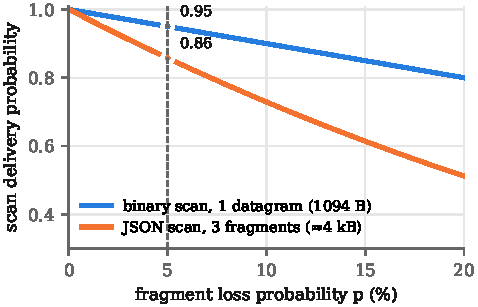
\includegraphics[width=0.5\textwidth]{packet_delivery.pdf}
\caption{Delivery probability of one LiDAR scan against per-fragment loss
(\cref{eq:frag}). At 5\% loss the single-datagram encoding arrives 95\% of the time,
against 86\% for the three-fragment JSON scan.}
\label{fig:delivery}
\end{figure}

\begin{figure}[H]
\centering
\begin{tikzpicture}[font=\scriptsize, x=1.1mm, y=1mm]
  \def\h{7}
  \draw[fill=blk1!20] (0,0)   rectangle (12,\h)  node[midway]{\texttt{'YDL1'}};
  \draw[fill=blk1!10] (12,0)  rectangle (36,\h)  node[midway]{capture $t$ (f64)};
  \draw[fill=blk1!20] (36,0)  rectangle (49,\h)  node[midway]{$N$ (u16)};
  \draw[fill=blk3!15] (49,0)  rectangle (104,\h) node[midway]{$N\times$ range in mm (u16)};
  \draw[fill=blk2!15] (104,0) rectangle (134,\h) node[midway]{$N\times$ intensity (u8)};
  \foreach \x/\l in {0/0,12/4,36/12,49/14,104/{14+2N},134/{14+3N}} \node[below] at (\x,0) {\l};
  \node[anchor=west] at (0,\h+3) {LiDAR datagram (UDP 14552), little-endian; byte offsets below};
  \begin{scope}[yshift=-19mm]
    \draw[fill=blk1!20] (0,0)  rectangle (22,\h)  node[midway, align=center]{meta length\\(u32)};
    \draw[fill=blk1!20] (22,0) rectangle (44,\h)  node[midway, align=center]{payload length\\(u32)};
    \draw[fill=blk1!10] (44,0) rectangle (92,\h)  node[midway, align=center]{JSON metadata: frame id,\\timestamp, shape, encoding};
    \draw[fill=blk3!15] (92,0) rectangle (134,\h) node[midway]{JPEG payload};
    \node[anchor=west] at (0,\h+3) {Camera frame on TCP 5000 (8-byte header, big-endian)};
  \end{scope}
\end{tikzpicture}
\caption{Wire formats of the LiDAR and camera streams.}
\label{fig:packets}
\end{figure}

\paragraph{Event-driven telemetry} ArduPilot's legacy \code{REQUEST_DATA_STREAM} groups
are limited to \SI{10}{\hertz}, which adds up to \SI{100}{\milli\second} of age. The
companion requests the five navigation messages (\code{ATTITUDE},
\code{LOCAL_POSITION_NED}, \code{OPTICAL_FLOW}, \code{RAW_IMU},
\code{DISTANCE_SENSOR}) at \SI{30}{\hertz} through
\code{MAV_CMD_SET_MESSAGE_INTERVAL}. The request is re-issued after the stream
requests, because ArduPilot resets per-message intervals when a group request is
applied. A packet is sent as soon as fresh navigation data arrive, after a
\SI{3}{\milli\second} coalescing window that merges one autopilot burst into one
packet. A \SI{200}{\milli\second} keep-alive covers quiet periods.
\Cref{fig:flow-telemetry} shows the loop.

\begin{figure}[H]
\centering
\begin{tikzpicture}[node distance=4.5mm]
  \node[term] (s) {start};
  \node[proc, below=of s] (w) {wait for nav-message event\\(timeout = keep-alive \SI{200}{\milli\second})};
  \node[proc, below=of w] (c) {coalesce \SI{3}{\milli\second}};
  \node[dec, below=of c] (g) {$\Delta t \ge 0.8/f_{\max}$?};
  \node[proc, below=of g] (p) {snapshot $\rightarrow$ drop stale ($>$\SI{1}{\second}) msgs\\$\rightarrow$ pack $\le$\SI{1400}{B} (rotate slow keys)};
  \node[proc, below=of p] (tx) {\code{sendto()} UDP 14551, DSCP CS6};
  \draw[arr] (s) -- (w);
  \draw[arr] (w) -- (c);
  \draw[arr] (c) -- (g);
  \draw[arr] (g) -- node[lbl,right]{yes} (p);
  \draw[arr] (p) -- (tx);
  \draw[arr] (g.east) -- node[lbl,above]{no: skip} ++(14mm,0) |- (w.east);
  \draw[arr] (tx.west) -- ++(-10mm,0) |- (w.west);
\end{tikzpicture}
\caption{Event-driven telemetry loop on the companion (\code{telemetry_streamer.py}).}
\label{fig:flow-telemetry}
\end{figure}

\paragraph{Wi-Fi QoS and power management} Telemetry, LiDAR and command packets carry
DSCP CS6 and video carries AF41. Under the RFC~8325 mapping \cite{rfc8325} these
are placed in the 802.11e/WMM voice and video access categories \cite{ieee80211e}, so
control traffic is not queued behind bulk video. Wi-Fi power saving is disabled on both
ends: when it is enabled, the station radio sleeps between beacons and buffers
incoming frames (commands, TCP ACKs) for \SIrange{10}{200}{\milli\second}.

\paragraph{Video without queueing} The camera thread drains the V4L2 queue
continuously with a driver buffer of one frame. The socket disables Nagle's algorithm
\cite{rfc896} and limits unsent data with \code{TCP_NOTSENT_LOWAT}. If the link is
still busy when a new frame is ready, that frame is \emph{dropped} rather than queued.
For control, a fresh frame is worth more than a complete sequence.
\code{--camera-passthrough} forwards the camera's own MJPEG bytes so the Pi does not
decode and re-encode.

\paragraph{Clock synchronisation and latency metrics} Every message carries the
sender's wall-clock capture time $t_s$. The receiver computes the raw one-way latency
and an \emph{excess} latency over a sliding \SI{10}{\second} window $W$:
\begin{equation}
  \ell_\text{raw}(k) = t_r(k) - t_s(k) - \delta_0, \qquad
  \ell_\text{excess}(k) = \ell_\text{raw}(k) - \min_{j\in W}\ell_\text{raw}(j).
  \label{eq:latency}
\end{equation}
$\ell_\text{raw}$ is absolute only when the clocks agree. \code{start_streams.py}
therefore makes the laptop the Pi's preferred \code{chrony} \cite{mills1991ntp}
source and steps the clock at start-up. $\ell_\text{excess}$ cancels any constant
offset and the fixed path delay, leaving queueing and Wi-Fi jitter. It is valid even
without synchronisation, and the health thresholds are applied to it
(warn \SI{150}{\milli\second}, error \SI{400}{\milli\second}). LiDAR scans are stamped
at the \emph{middle} of the revolution, $t_s=\tfrac12(t_\text{start}+t_\text{end})$,
because the samples are spread over the whole turn.

\paragraph{Revolution segmentation} The G2 firmware (v3.5) sets its "start of scan"
flag only every 3--4 revolutions. We saw only 2 flags per second at 6.4 rev/s. Relying on it merged several turns into one \SI{2}{\hertz} scan about
\SI{200}{\milli\second} old. The streamer instead detects a new revolution when the
packet start angle wraps, $\theta_\text{start} + 180^\circ < \theta_\text{start,prev}$.

\subsection{Odometry reconstruction without GNSS}
\label{sec:design-odom}

\paragraph{Source selection} \code{mavlink_to_ros2_bridge} publishes
\topic{/odom} and the \code{odom}$\rightarrow$\code{base_link} transform. If the
autopilot's EKF publishes \code{LOCAL_POSITION_NED}, that fused estimate is used
directly. Otherwise horizontal position is dead-reckoned from optical flow. Any
navigation message older than \SI{1}{\second} is treated as absent, so a sensor that
stops cannot freeze a stale position into the map.

\paragraph{Frame conversion} With NED position $(n,e,d)$ and ArduPilot Euler angles
$(\phi,\theta,\psi)$, $\psi$ clockwise from north, the ROS quantities are
\begin{equation}
  (x,y,z)_\text{ENU} = (e,\,n,\,-d), \qquad
  (\phi,\theta,\psi)_\text{ROS} = \left(\phi,\,-\theta,\,\operatorname{wrap}\!\left(\tfrac{\pi}{2}-\psi\right)\right).
  \label{eq:ned-enu}
\end{equation}

\paragraph{Optical-flow velocity} The MAVLink specification defines
\code{OPTICAL_FLOW.flow_comp_m_x/y} as metric velocity. ArduPilot instead fills them with
gyro-compensated angular flow rates $\omega_x,\omega_y$ (\si{\radian\per\second}),
each a rotation \emph{about} that axis. Following ArduPilot's EKF3 flow model, the
body-frame (FRD) velocity at height $h$ is
\begin{equation}
  v_{x}^{\text{FRD}} = -\,\omega_y\,h, \qquad v_{y}^{\text{FRD}} = \omega_x\,h,
  \label{eq:flow-ap}
\end{equation}
with $h$ taken from the flow message's ground distance, or from the rangefinder when
that is zero (as it is indoors without an EKF origin). For the integrated
\code{OPTICAL_FLOW_RAD} message, the gyro-integrated body rotation is subtracted
first: $v_x = (\Theta_y - \Gamma_y)h/\Delta t$ and
$v_y = -(\Theta_x - \Gamma_x)h/\Delta t$. Samples with quality below 20/255 are
discarded. The FRD$\rightarrow$FLU change negates $v_y$, and the body velocity is
rotated into the world frame by the ROS yaw $\psi_r$ and integrated:
\begin{equation}
  \begin{bmatrix} x \\ y \end{bmatrix}_{k+1} =
  \begin{bmatrix} x \\ y \end{bmatrix}_{k} +
  \begin{bmatrix} \cos\psi_r & -\sin\psi_r \\ \sin\psi_r & \cos\psi_r \end{bmatrix}
  \begin{bmatrix} v_x \\ -v_y \end{bmatrix}^{\!\text{FRD}} \Delta t_k ,
  \qquad 0 < \Delta t_k < \SI{1}{\second}.
  \label{eq:flow-integrate}
\end{equation}

\paragraph{Zero-velocity update (ZUPT)} Integrating noisy flow at rest produces drift. Following the
zero-velocity-detection literature \cite{foxlin2005pedestrian,skog2010zupt}, the
bridge declares the vehicle stationary when, over a window $W$ of
\SI{1}{\second} containing at least five samples spanning at least \SI{0.6}{\second},
\begin{equation}
  \sigma_W\!\left(\lVert\mathbf{f}\rVert\right) < \SI{15}{\milli\gacc}
  \quad\text{and}\quad
  \overline{\lVert\bm{\omega}\rVert}_W < \SI{4}{\degree\per\second},
  \label{eq:zupt}
\end{equation}
where $\mathbf{f}$ is specific force and $\bm{\omega}$ angular rate. While stationary,
or when telemetry is older than \SI{0.5}{\second} (a Wi-Fi drop-out), the integrated
velocity is forced to zero and position holds. The thresholds were chosen from a bench
log ($\sigma\approx\SI{3}{\milli\gacc}$, $\approx\SI{1}{\degree\per\second}$) and are
far below hover vibration levels. \Cref{sec:val-zupt} evaluates them.

\paragraph{Height source} With the bridge parameter \code{z_source} set to \code{auto}, height is taken from the first
available of: dedicated rangefinder, the flow module's ground distance (only when its
quality is sufficient), EKF local $-d$, and barometric altitude relative to the first
reading after start-up. Barometric altitude uses the standard-atmosphere relation
\cite{icao1993atmosphere}
\begin{equation}
  h_\text{baro} = 44\,330\left[1-\left(\frac{p}{1013.25\,\text{hPa}}\right)^{0.190295}\right]\ \text{m}.
  \label{eq:baro}
\end{equation}

\subsection{Planning and control}

\paragraph{Costmaps} Both costmaps are rolling windows in \code{odom}, so no prior map
or global localisation is needed. The local map is $8\times8$\,m at
\SI{5}{\hertz} and the global map $20\times20$\,m at \SI{1}{\hertz}, both at
\SI{0.05}{\metre} resolution. Obstacle marking and ray-tracing use \topic{/scan} over
\SIrange{0.10}{8.0}{\metre}. The \SI{8}{\metre} cap reflects the G2's reduced
reliability beyond that range indoors. The footprint radius is \SI{0.25}{\metre},
and cost decays outside it as Nav2's exponential inflation
\begin{equation}
  c(d) = 252\, e^{-\kappa\,(d - r_\text{robot})}, \qquad
  r_\text{robot} < d \le r_\text{infl},
  \label{eq:inflation}
\end{equation}
with $\kappa=3.0$ and $r_\text{infl}=\SI{0.40}{\metre}$.

\paragraph{Controller} The DWB local planner \cite{fox1997dwa} at \SI{10}{\hertz} is
configured as a \emph{holonomic} vehicle. Lateral velocity is sampled (15$\times$15
samples) over $\pm\SI{0.5}{\metre\per\second}$ with
\SI{0.5}{\metre\per\second\squared} acceleration limits, and yaw rate is fixed at zero:
a multirotor can translate in any direction without turning. Critics are
\code{Oscillation}, \code{BaseObstacle}, \code{PathAlign}, \code{PathDist} and
\code{GoalDist}. Yaw goal tolerance is effectively disabled
(\SI{3.15}{\radian}) and the $xy$ tolerance is \SI{0.20}{\metre}.

\paragraph{Behaviour tree for a flying base} Nav2's default recoveries (spin, back up)
are useless or harmful here: in simulation, backing up flew into the \SI{270}{\degree}
LiDAR's blind sector and hit a wall. The custom tree \code{navigate_drone.xml} replaces them with
costmap clearing followed by a \SI{3}{\second} hover, retried up to six times
\cite{colledanchise2018bt}.

\paragraph{Velocity command transformation} Nav2 emits body-frame (FLU) velocity
$(v_x,v_y,v_z,\dot\psi)$. The companion converts it to the
\code{SET_POSITION_TARGET_LOCAL_NED} setpoint using the latest autopilot heading
$\psi$ (clockwise from north):
\begin{equation}
  \begin{aligned}
  v_N &= \cos\psi\,v_x + \sin\psi\,v_y, &\quad v_E &= \sin\psi\,v_x - \cos\psi\,v_y,\\
  v_D &= -v_z, & \dot\psi_\text{NED} &= -\dot\psi ,
  \end{aligned}
  \label{eq:cmd}
\end{equation}
with \code{type_mask} $=1479$ (\texttt{0b010111000111}), so position, acceleration and
absolute yaw are ignored and velocity and yaw rate are used. If no heading has been
received, no setpoint is sent; the code does not guess.

\subsection{Layered safety design}
\label{sec:design-safety}

Safety is enforced at several independent layers (\cref{fig:safety}), so no single
software fault can command unsafe motion:
\begin{enumerate}[leftmargin=*,itemsep=1pt]
  \item \textbf{Human authority.} Arming and take-off are performed by the pilot on
    the RC transmitter. The laptop never auto-arms (\code{auto_arm=false}), and the
    listener forwards velocity \emph{only} while the vehicle is armed and in
    \code{GUIDED}. Switching the RC mode switch out of \code{GUIDED} returns control to
    the pilot immediately.
  \item \textbf{Speed envelope.} The ground bridge clamps horizontal speed to
    $\lVert(v_x,v_y)\rVert\le\SI{0.5}{\metre\per\second}$ by scaling the vector,
    which preserves its direction. The DWB limits are the same.
  \item \textbf{Liveness.} The ground bridge sends a stop when \topic{/cmd_vel} is older
    than \SI{0.5}{\second}. The Pi discards commands older than \SI{1}{\second}. The
    bridge publishes \code{/odom} at a \SI{10}{\hertz} fallback rate during drop-outs,
    so TF stays valid while position holds.
  \item \textbf{Vibration guard} (\code{vibration_motor_halt.py}, bench/optional). When
    vibration exceeds \SI{35}{\metre\per\second\squared}, it overrides the RC channels
    to \SI{40}{\percent} throttle (PWM \SI{1400}{\micro\second}) with level
    attitude, ignores stick input, and offers emergency disarm.
  \item \textbf{Autopilot failsafes.} RC-loss and low-battery actions configured in
    ArduPilot operate regardless of the companion.
\end{enumerate}

\begin{figure}[t]
\centering
\begin{tikzpicture}[node distance=4mm]
  \node[term] (in) {\topic{/cmd_vel} from Nav2};
  \node[proc, below=of in] (clamp) {ground: clamp $\lVert v_{xy}\rVert \le \SI{0.5}{\metre\per\second}$};
  \node[dec, below=of clamp] (fresh) {age $< \SI{0.5}{\second}$?};
  \node[proc, right=14mm of fresh] (stop) {send zero velocity};
  \node[proc, below=of fresh] (udp) {UDP 14553 $\rightarrow$ Pi listener};
  \node[dec, below=of udp] (armed) {armed $\wedge$ \code{GUIDED}?};
  \node[proc, right=14mm of armed] (drop) {do not forward\\(pilot in control)};
  \node[dec, below=of armed] (age) {cmd age $<\SI{1}{\second}$\\$\wedge$ heading known?};
  \node[proc, below=of age] (conv) {FLU$\rightarrow$NED (\cref{eq:cmd})};
  \node[term, below=of conv] (out) {\code{SET_POSITION_TARGET_LOCAL_NED}};
  \draw[arr] (in) -- (clamp);
  \draw[arr] (clamp) -- (fresh);
  \draw[arr] (fresh) -- node[lbl,right]{yes} (udp);
  \draw[arr] (fresh) -- node[lbl,above]{no} (stop);
  \draw[arr] (stop) |- (udp);
  \draw[arr] (udp) -- (armed);
  \draw[arr] (armed) -- node[lbl,right]{yes} (age);
  \draw[arr] (armed) -- node[lbl,above]{no} (drop);
  \draw[arr] (age) -- node[lbl,right]{yes} (conv);
  \draw[arr] (age.east) -| node[lbl,pos=0.25,above]{no} (drop.south);
  \draw[arr] (conv) -- (out);
\end{tikzpicture}
\caption{Command-path safety gating from Nav2 to the autopilot. The Pi re-evaluates
the gate on every new command and at a \SI{20}{\hertz} keep-alive.}
\label{fig:safety}
\end{figure}

\paragraph{Simulation-only LiDAR safety filter} In the PX4 simulation bridge, each
LiDAR return $i$ within reach $r_i\le r_\text{reach}=\SI{0.65}{\metre}$, with unit
bearing $\hat{\mathbf{u}}_i$, removes the commanded velocity component towards it:
\begin{equation}
  \mathbf{v} \leftarrow \mathbf{v} - \max\!\left(0,\ \mathbf{v}\cdot\hat{\mathbf{u}}_i\right)\hat{\mathbf{u}}_i ,
\end{equation}
applied in two passes. Returns closer than $r_\text{hard}=\SI{0.45}{\metre}$ add a
repulsion $-\sum_i (1-r_i/r_\text{hard})\,\hat{\mathbf{u}}_i$, scaled to at most
\SI{0.15}{\metre\per\second}. Unlike an earlier stop-all version, which froze the drone beside door frames, the
projection lets it slide along walls and back out of doorways. The same bridge yaws the vehicle towards
its direction of travel, because the simulated LiDAR is blind over the rear
\SI{90}{\degree}. Speed is scaled by $\max(0.25,\cos e_\psi)$ while turning, and by
0.1 when the heading error exceeds \SI{90}{\degree}.

\subsection{Hybrid semantic perception}
\label{sec:design-perception}

YOLOv8 instance segmentation \cite{redmon2016yolo,jocher2023yolov8} provides classes,
confidences and boxes in a few milliseconds. Its masks, however, are decoded from a
low-resolution prototype grid and are coarse at object boundaries. Segment Anything
\cite{kirillov2023sam,ravi2024sam2} produces sharp, class-agnostic masks when prompted.
The hybrid segmenter prompts SAM~2.1 with YOLO's boxes, so one image encoding is shared
by all instances. It then accepts each SAM mask only if four gates pass
(\cref{fig:seg-flow}). Otherwise it keeps the YOLO mask:
\begin{enumerate}[leftmargin=*,itemsep=1pt]
  \item SAM's predicted-IoU score $\ge 0.5$;
  \item the mask is clipped to the YOLO box grown by a 10\% margin (prevents leakage);
  \item the mask fills $\ge 5\%$ of the box (rejects slivers);
  \item $\text{IoU}(M_\text{SAM}, M_\text{YOLO}) \ge 0.3$ when a YOLO mask exists, which
    rejects SAM selecting a different object or a sub-part (e.g.\ a shirt instead of
    the person), where $\text{IoU}(A,B)=|A\cap B|/|A\cup B|$.
\end{enumerate}
Label images are rasterised from the largest mask to the smallest, so small objects on
top of large ones survive, and ties go to the more confident detection. YOLO runs in
FP16 on CUDA. SAM~1-family models are kept in FP32, because we got
empty masks from them in half precision. The default in the full stack is SAM at \SI{768}{px}: we
measured \SI{36}{\milli\second} inference and \SI{46}{\milli\second}
capture-to-result on the drone feed, against \SI{50}{\milli\second}/\SI{60}{\milli\second}
at \SI{1024}{px}, with near-identical masks.

\begin{figure}[H]
\centering
\begin{tikzpicture}[node distance=4mm and 6mm]
  \node[term] (f) {frame (BGR)};
  \node[proc, right=of f, minimum width=26mm] (y) {YOLOv8n-seg\\boxes, classes, masks};
  \node[proc, right=of y, minimum width=26mm] (s) {SAM 2.1\\box prompts};
  \node[dec, below=6mm of s] (g) {4 gates\\pass?};
  \node[proc, left=10mm of g, minimum width=22mm] (ky) {keep YOLO\\mask \code{[Y]}};
  \node[proc, right=8mm of g, minimum width=22mm] (ks) {use SAM\\mask \code{[S]}};
  \node[proc, below=7mm of g, minimum width=40mm] (r) {rasterise large$\rightarrow$small:\\class \& instance masks};
  \draw[arr] (f) -- (y);
  \draw[arr] (y) -- (s);
  \draw[arr] (s) -- (g);
  \draw[arr] (g) -- node[lbl,above]{no} (ky);
  \draw[arr] (g) -- node[lbl,above]{yes} (ks);
  \draw[arr] (ky) |- (r);
  \draw[arr] (ks) |- (r);
\end{tikzpicture}
\caption{Hybrid segmentation pipeline (\code{hybrid_segmenter.py}).}
\label{fig:seg-flow}
\end{figure}

\subsection{3D mapping from a 2D LiDAR}

\code{scan_to_3d} turns each horizontal scan into 3D points using the full
time-matched transform $\,^{o}\mathbf{T}_{l}(t)= {}^{o}\mathbf{T}_{b}(t)\,{}^{b}\mathbf{T}_{l}$
(height, roll, pitch, yaw and mount), so slices taken at different heights stack
into a volumetric map. Points fall into a \SI{5}{\centi\metre} voxel grid. A voxel is
published after two hits, and scans are skipped while tilt exceeds
\SI{30}{\degree}. The map is published at \SI{1}{\hertz} and saved as PLY. Its fidelity
is bounded by the height estimate and by horizontal flow drift.

\subsection{Observability: health metrics}

\code{metrics_monitor} republishes scalar health signals under \topic{/metrics/*}
(rates, jitter, latency, decode time, bandwidth, nearest obstacle, TF age, plan length,
command speed, CPU) and aggregates OK/WARN/FAIL into \topic{/diagnostics} and an RViz
overlay. One metric checks the whole TF and timing chain end to end. The
\emph{scan agreement} $\alpha$ is the fraction of LiDAR returns inside the local
costmap whose cell, or a direct neighbour, is lethal (value 100 in the published
\code{OccupancyGrid}):
\begin{equation}
  \alpha = \frac{\left|\{\,i : \max_{c\in\mathcal{N}_8(\text{cell}(\mathbf{p}_i))\cup\{\text{cell}(\mathbf{p}_i)\}} C(c) = 100\,\}\right|}{\left|\{\,i : \mathbf{p}_i \in \text{costmap}\}\right|}.
  \label{eq:agreement}
\end{equation}
Values of $\alpha\approx1$ show that the costmap reproduces what the LiDAR sees. A
drop reveals a wrong mount transform, stale TF or dropped scans.
